% All numbers recomputed 2026-08-25 on the 120-column extractor in
% canonical-depth pose mode (mode C, docs/FEATURE_AUDIT.md 5.7), from
%   experiments/feature_validity/results/reference_validity.csv
%   mm_fusion_top50/combined_data/phenotypes_v2.csv        (patients, arm C)
%   chop_22q_analysis/feats_fairface_v2/phenotypes_all.csv (reference, arm C)
% The superseded arm-D matrices sit beside each as *.armD_perimage_z.bak.csv.
%
% Requires in the preamble:
%   \usepackage{graphicx}
%   \usepackage{subcaption}
% Figures are expected in ./image/ .

\subsection{Quantitative measurements reproduce annotated facial phenotypes}

We applied FaceKit to a curated subset of the GestaltMatcher Database comprising
4,559 frontal facial images from 50 rare-disease cohorts. For each image, FaceKit
extracted 478 facial landmarks and computed 120 unitless geometric measurements.
After pose filtering and collapsing each patient to the median of their frontal
images, 2,897 patients remained. To express every measurement on a common,
clinically interpretable scale, we built a normative reference from 2,051 FairFace
control images spanning three ancestry groups, of which 886 passed the same pose
filter, and converted each measurement into a $z$-score relative to that reference.
Each of the 97 facial HPO terms in the FaceKit vocabulary is mapped to one
measurement together with the direction in which that measurement is expected to
change, so a signed $z$-score can be read directly as agreement or disagreement
with the annotation.

Of the 97 terms, 84 were carried by at least one patient with a gold-standard
annotation; the remaining 13 had no annotated patient anywhere in the cohort and
could not be assessed. Across the 84 assessable terms, the mapped measurement
deviated from the healthy reference in the direction predicted by HPO for 62
(73.8\%; binomial $p=1.5\times10^{-5}$), with a mean absolute deviation of 0.47
reference standard deviations. Restricting attention to the 78 terms carried by
enough patients to admit a statistical test, 33 reached significance after
Benjamini--Hochberg correction, 39 did not separate from the reference, and 6
deviated significantly in the direction opposite to the one HPO predicts. Agreement
was not driven by the terms with the most annotation: terms carried by 10--29
patients agreed as often as those carried by 30 or more (82.4\% versus 79.5\%).

Hypertelorism illustrates how an individual measurement can be read. The term is
mapped to the inter-pupillary distance normalized by bizygomatic width, the ratio
of the distance between the two iris centres to the distance between the two
zygomatic points (Fig.~\ref{fig:ipd}\subref{fig:ipd-crouzon},\subref{fig:ipd-costello}). Across the 238 patients annotated with the term,
this ratio was elevated by 1.04 reference standard deviations
($q=4.2\times10^{-22}$), and among all 120 measurements it was the most
deviant in these same patients, indicating that the signal is specific to the
measurement the term is mapped to rather than a general distortion of the face.
The same ordering is visible at the cohort level: mean normalized inter-pupillary
distance was 0.532 in the Crouzon syndrome cohort against 0.465 across the
remaining cohorts, the highest of the 50 diseases (Fig.~\ref{fig:ipd}\subref{fig:ipd-bars}). Panels \subref{fig:ipd-crouzon} and \subref{fig:ipd-costello} contrast a Crouzon patient with a patient from a cohort at the centre of the same
distribution, with the two landmark pairs entering the ratio drawn on the image.

\begin{figure}[t]
  \centering
  \begin{subfigure}[b]{0.48\linewidth}
    \centering
    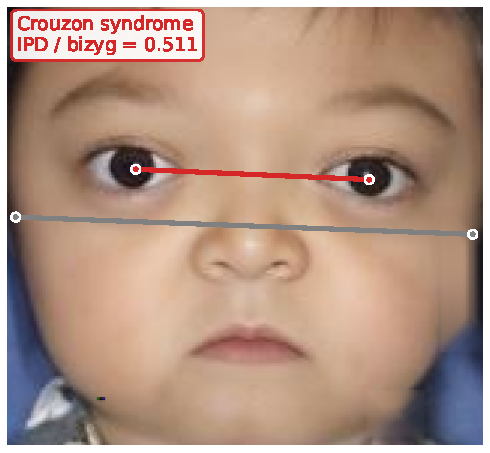
\includegraphics[width=\linewidth]{image/F1a_face_crouzon}
    \caption{}
    \label{fig:ipd-crouzon}
  \end{subfigure}
  \hfill
  \begin{subfigure}[b]{0.48\linewidth}
    \centering
    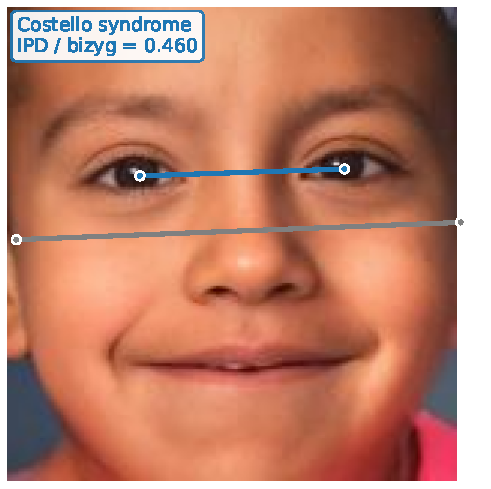
\includegraphics[width=\linewidth]{image/F1b_face_costello}
    \caption{}
    \label{fig:ipd-costello}
  \end{subfigure}

  \vspace{1em}

  \begin{subfigure}[b]{0.85\linewidth}
    \centering
    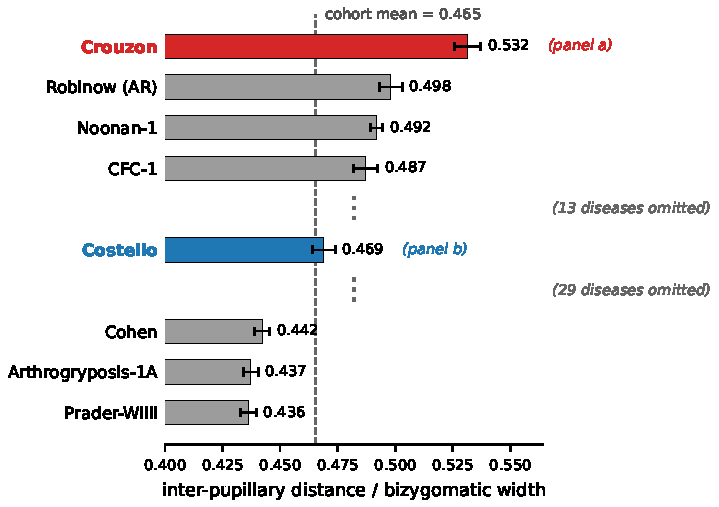
\includegraphics[width=\linewidth]{image/F1c_ipd_bars}
    \caption{}
    \label{fig:ipd-bars}
  \end{subfigure}

  \caption{\textbf{A single FaceKit measurement, from image to cohort.}
  (\subref{fig:ipd-crouzon}, \subref{fig:ipd-costello}) The inter-pupillary
  distance normalized by bizygomatic width, drawn on the images it is computed
  from: the coloured line joins the two iris centres (landmarks 468 and 473) and
  the grey line joins the two zygomatic points (landmarks 234 and 454); the
  measurement is the ratio of their lengths. (\subref{fig:ipd-crouzon}) A patient
  with Crouzon syndrome, the cohort with the highest mean value.
  (\subref{fig:ipd-costello}) A patient with Costello syndrome, a cohort at the
  centre of the same distribution, shown for contrast.
  (\subref{fig:ipd-bars}) Mean normalized inter-pupillary distance per disease
  cohort. Bars give the cohort mean with its standard error; the dashed line marks
  the mean over the remaining cohorts. Of the 50 cohorts, the four highest, the
  three lowest and Costello syndrome are shown, and the rest are omitted as
  indicated. Values are computed on images passing the frontal-pose filter.}
  \label{fig:ipd}
\end{figure}

The six measurements that moved against their annotation share a single
explanation, and it is not that the annotations are wrong. In each case the
annotated patients were barely distinguishable from the patient cohort as a whole:
patients annotated with a narrow nasal bridge measured $+0.82$ against a
cohort-wide baseline of $+0.53$, facial asymmetry $-0.63$ against $-0.48$, and full
cheeks $-0.65$ against $-0.56$. For the other three the annotated patients were in
fact closer to the reference than the average patient: synophrys $+0.41$ against
$+0.52$, a narrow forehead $+0.37$ against $+0.56$, and ptosis $+0.16$ against
$+0.35$. These are therefore not phenotype effects with an inverted sign but
cohort-wide offsets in the measurement itself, which happen to point away from the
direction the term predicts.

Each offset has an identifiable source. Every asymmetry measurement, not only the
one mapped to facial asymmetry, was systematically lower in patients than in
controls (13 of 14 such columns negative, mean $-0.27$). This is a property of the
reference rather than of the patients: an asymmetry measurement is driven by
whatever head pose survives the frontal gate (mean $r=+0.45$ against $|$yaw$|$
across the 15 asymmetry columns), and the FairFace controls carry more residual
pose than the patient photographs do after the same gate (mean $|$yaw$|$
$6.1^{\circ}$ against $4.1^{\circ}$). Stratified by $|$yaw$|$ the two populations
almost coincide (0--3$^{\circ}$: 0.032 against 0.037; 3--6$^{\circ}$: 0.050
against 0.055; 6--9$^{\circ}$: 0.074 against 0.081), so the apparent deficit is
the reference being measured under looser acquisition conditions, not a face that
is genuinely more symmetric. Cheek area is normalized by the square of bizygomatic width, and the
patients annotated with full cheeks did have broader and rounder faces
(face aspect ratio $+0.34$, roundness $+0.29$ against cohort baselines of $+0.07$
and $+0.11$); the denominator therefore grows with the phenotype and inverts the
ratio, the same failure mode that normalization by a phenotype-sensitive scale
produces elsewhere. For synophrys, the measurement is the gap between the medial
brow endpoints, but synophrys is hair occupying that gap, and the landmark mesh
carries no photometric information: the brow points are placed by the shape prior
rather than by the hair boundary. Consistent with this, the brows of these patients
did differ from the reference in shape, but in a different measurement
(medial flare $-0.75$) than the one the term is mapped to. The two weakest cases
are weak for reasons that are visible in the result itself: for ptosis the mapped
measurement ranks 88th of the 120 in these patients, so it is not among the
measurements that deviate at all and reaches significance only through the number
of patients carrying the term ($n=138$), while a narrow forehead is significant
only marginally ($q=0.047$) and is measured from landmarks that lie under the
hairline, where the mesh has no image evidence to place them and where residual
pose dependence remains high ($|r|=0.46$ against pitch, 12th of the 120
measurements). Only the
narrow nasal bridge result rests on few patients ($n=19$), and it uses landmark
indices that have not been verified against the canonical face model.

These six cases indicate that a measurement should be interpreted against the
patient population as well as against healthy controls, since a cohort-wide offset
can produce a confident result in either direction, and that normalization scales
must be chosen so that the denominator is not itself altered by the phenotype being
measured.
